\documentclass[conference,9pt]{IEEEtran}
\usepackage{xcolor}
\usepackage{cite}
\usepackage{epsfig}
\usepackage{amssymb}
\usepackage{amsmath}
\usepackage{graphicx}
\graphicspath{ {./} }

\begin{document}
\title{Practical 3b}

\author{
\IEEEauthorblockN{Albert Acebron}
\IEEEauthorblockA{NIU: 1458626}
}


% make the title area
\maketitle
\begin{abstract}
In this practical we will analyse the spectral estimate of a GNSS signal and study it's properties.
\end{abstract}

\section{Periodograms}
Let's start by modifying our previous compute\_periodogram function to make sure that the returned value has a frequency resolution of 0.00001. To achieve this we will make sure that the fft computed within the function returns a vector of $\frac{1}{0.00001}=10^5$.

\begin{verbatim}
  function S_per = compute_periodogram(signal)
    N=length(signal);
    S_per=abs(fft(signal, 1e5)).^2/N;
  end
\end{verbatim}

Applying this function to our signal\footnote{See appendix for the code used here} we get the following result:

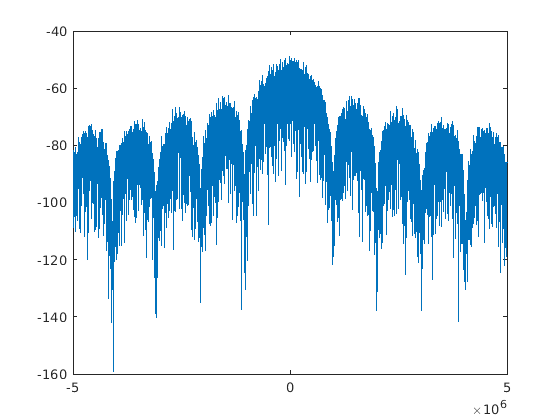
\includegraphics[scale=0.5]{b1}

Which we can then compare against the periodograms of the two ideal GNSS signals:

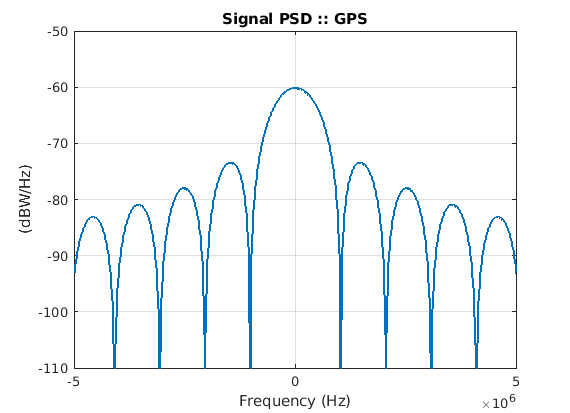
\includegraphics[scale=0.6]{gps}

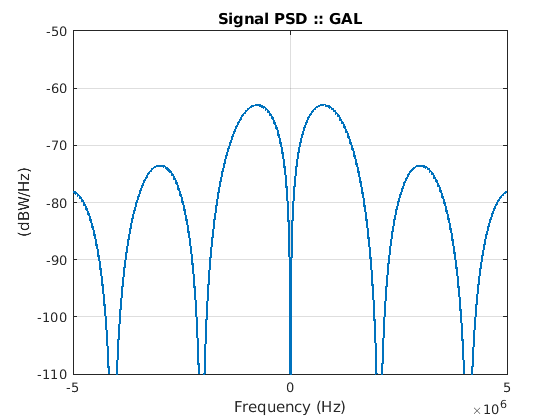
\includegraphics[scale=0.6]{gal}

It's easy to see that our signal is a GPS one, as it has one big lobe at frequency 0. Furthermore if we superpose both graphs we can see that they match:

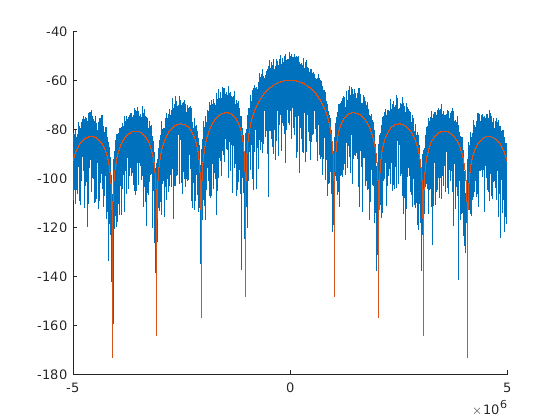
\includegraphics[scale=0.6]{compare}

\section{Bias}
To start our study on the bias present in our calculation let's assume that we are dealing with a constant function.

Now, taking into account equation (1.4) from the practical:
$$E(S^{(per)})=W(e^{jw})*S_x(e^{jw})$$

where $w(m)=1-\frac{|m|}{N}$.

Because the function under study is constant, it's autocorrelation will also be a constant function and the fourier transform of that will be a delta at frequency 0\footnote{This is just a direct consequence of applying the transform}, which means that $S_x(e^{jw})=\delta(e^{jw})$.

Taking this result we can follow the properties of the convolution and we will get that 
$$E(S^{(per)})=W(e^{jw})*\delta(e^{jw})=W(e^{jw})$$

Which means that the estimation of our periodogram will be equal to the fourier transform of $w(m)$.

At this point we could just calculate analytically what's the FT of the triangle function $w$, which would lead us to $sinc^2$. However, instead of doing that we will do calculate it numerically, by plotting the FT of triangle functions of different lengths:

Length 100:

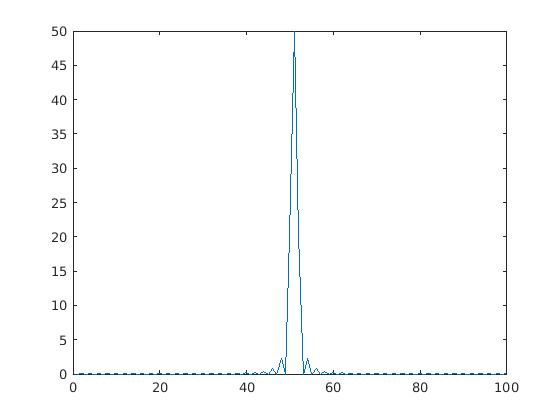
\includegraphics[scale=0.6]{triang100.png}

Length 1000:

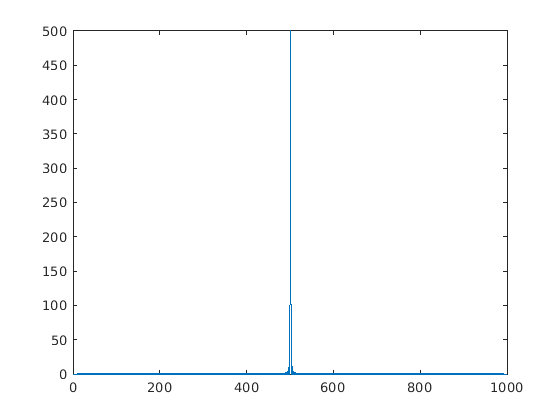
\includegraphics[scale=0.6]{triang1000.png}

As we can see, the higher the length the closer the resulting function is to a delta, with the most power concentrated on frequency 0. This is quite interesting because if the signal that we are manipulating is convoluted by this, so if it takes the form of a delta (which happens at $N=\infty$) the estimated periodogram will unaffected by the convolution and the estimation will be unbiased.

However, because when $N<\infty$ it's not actually a delta and it has non-zero values at frequencies other than zero, the convolution will create shifted copies of the periodogram that will be all summed together to form the estimation\footnote{This is easy to see if we descompose the $sinc^2$ function into a sum of deltas and use the linearity of convolution, as in that case we will end up with a sum of shifted signals}. Practically, this means that in our estimated periodogram we may see values at frequencies where the actual periodogram is zero, a phenomenon called power leakage.

In conclusion, the more samples we use for our estimation, the closer it will be to the real periodogram, as the influence that processes such as power leakage have over the final result will be lowered.

With that said, we will evaluate how this affects our previous estimates by taking samples of different length and comparing several metrics between them.

\subsection{Sample of $50\mu s$ (500 data points)}
Periodogram:

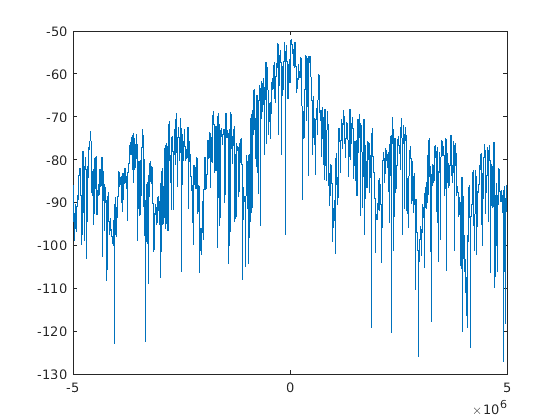
\includegraphics[scale=0.6]{perio500.png}

Error:

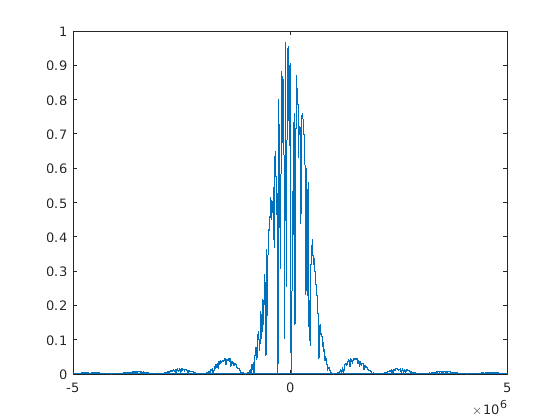
\includegraphics[scale=0.6]{error50.png}

\subsection{Sample of $500\mu s$ (5000 data points)}

Periodogram:

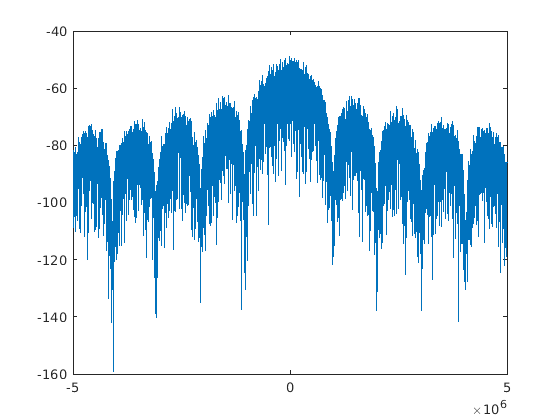
\includegraphics[scale=0.5]{b1}

Error:

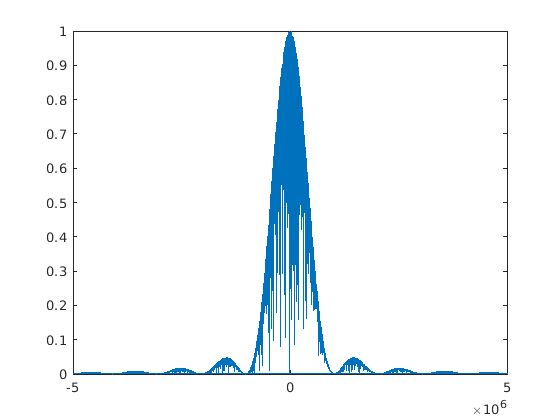
\includegraphics[scale=0.6]{error500.png}

As we can see, the higher the number of samples, the closer the periodogram is to it's real values.

In terms of the error, we see very similar results for both cases, which shouldn't happen since the longer sample should have lower error due to the fact that this estimation has a lower bias compared to the estimation that uses less data points (we saw this in the previous section). However, in this case we don't see that happening, so I think that I've made a mistake somewhere.

\section{Variance}
In this section we will start delving more into an analysis of the main lobe, which, as we can appreciate in the following plot, is located between -1MHz and 1MHz in the ideal spectrum:

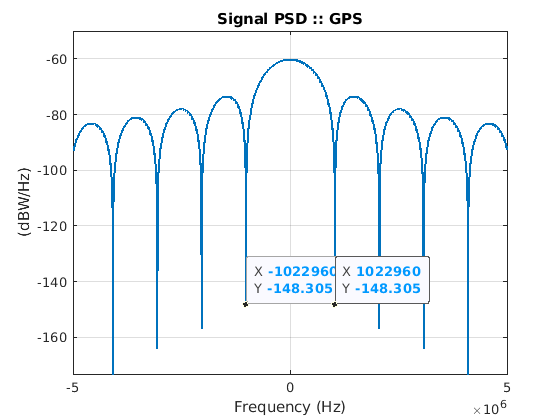
\includegraphics[scale=0.6]{mainlobe.png}

In the beginning of this practical we made sure that the frequncy resolution on which we operate is $10^{-5}$, which means that in total the periodograms that we plot have $10^{5}$ points. As these are distributed evenly in the [-5MHz, 5MHz] frequency range, the point where the main lobe starts will be the $4\cdot 10^4$th, situated at -1MHz, and the point where it ends is the $6\cdot 10^4$th.

Note that this assumes that fftshift has been applied to the result, in case it hasn't, the ranges that hold the main lobe would be [0, 1e4]U[9e4, 1e5].

We can use this now to isolate the errors of our estimation in the main lobe and compute the variance of the resulting vector:

\begin{center}
  \begin{tabular}{ c c }
   N & variance \\ 
   500 &  0.0769 \\  
   5000 & 0.0951    
  \end{tabular}
\end{center}

It seems that variance of the error doesn't change much with the amount of data processed (it only increases slightly with a higher amount of data). This means that our estimator is not consistent, as an increase of data points doesn't lead to a decrease in variance.

\section{Bartlett's method}
We'll compute various Barlett estimations using different values for L\footnote{See appendix for code}:

\subsection{L=2}
Comparison:

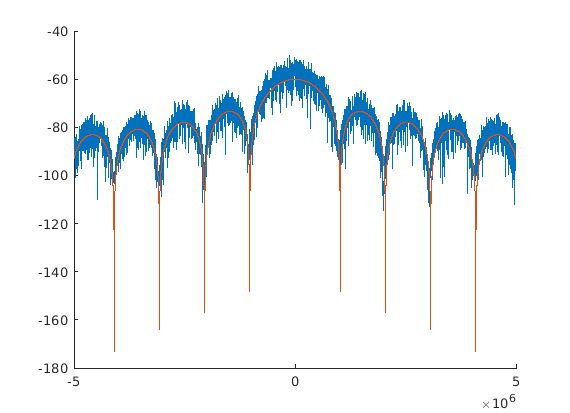
\includegraphics[scale=0.6]{barlett2.png}

Error:

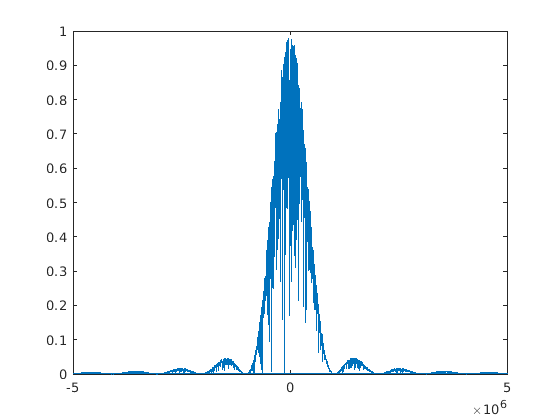
\includegraphics[scale=0.6]{me2.png}

\subsection{L=10}
Comparison:

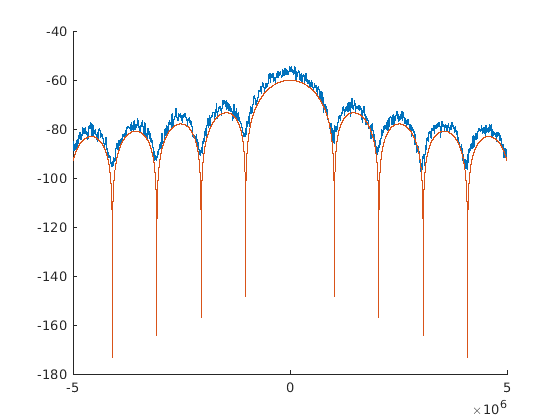
\includegraphics[scale=0.6]{barlett10.png}

Error:

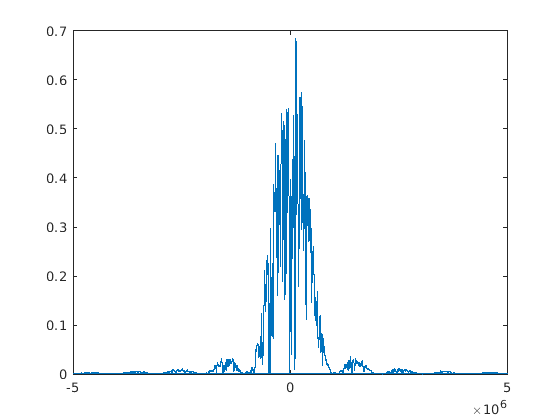
\includegraphics[scale=0.6]{me10.png}

\subsection{L=50}
Comparison:

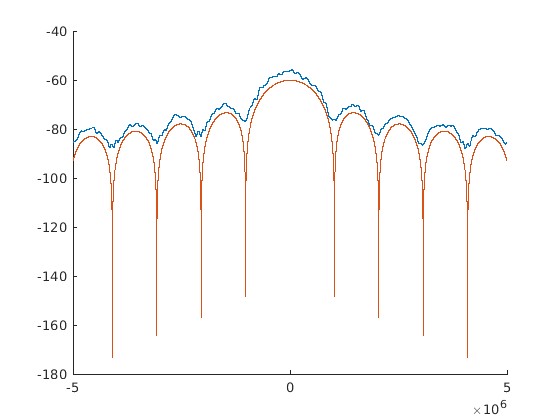
\includegraphics[scale=0.6]{barlett50.png}

Error:

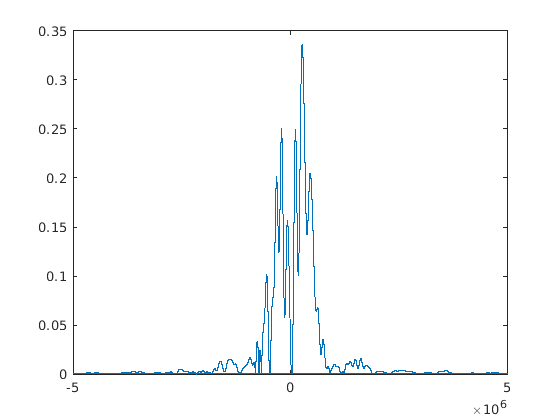
\includegraphics[scale=0.6]{me50.png}

Following our example from before we'll also compute the variance of the error at the main lobe:

\begin{center}
  \begin{tabular}{ c c }
   L & variance \\
   2 &  0.0822 \\
   10 &  0.0275 \\
   50 & 0.0074    
  \end{tabular}
\end{center}

Generally the trend seems to be that the an increase in the value of $L$ causes a decrease of variance at the cost of an increase in the bias.

% The decrease in bias can be explained by saying that, because now we are averaging multiple estimations of the same value, this average will tend to be closer to the expected value that the estimator provides, and thus the bias will be lower. In other words, averaging a lot of the noise/jitter in the estimation (as seen in previous practicals) and this brings the values closer to the expected ones (the expected values are still biased since we are using a biased estimator here, but that bias is much lower than the error caused by jitter/noise).

The decrese in variance is a direct consequence of the equation (2.1) provided in the practical. An intuitive explanation of this is that by averaging multiple results we get a value closer to the expected one, and as the variance is defined as the squared difference between these, making that smaller causes the variance to get lower aswell.

The increase in bias is caused by the fact that our estimations now use less samples, which decreases the spectral resolution, thus leading to an increase in bias.

\section{AR estimation}
Next we will change our estimator for an AR one and see how it responds for different values of p:

\subsection{p=10}
Comparison:

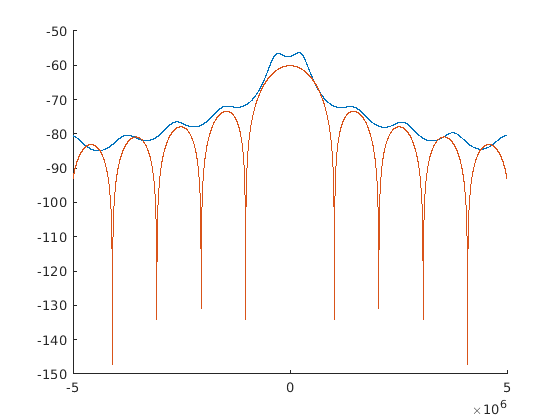
\includegraphics[scale=0.6]{arp10.png}

Error:

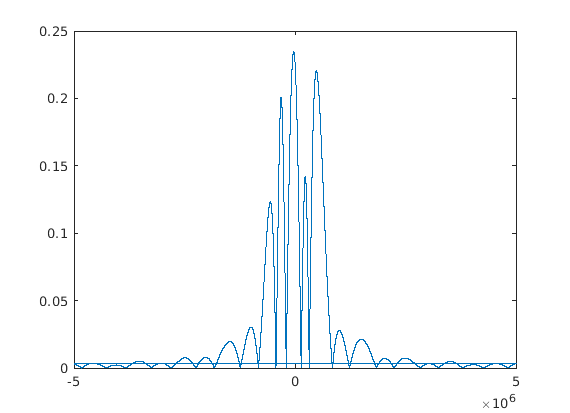
\includegraphics[scale=0.6]{earp10.png}

\subsection{p=100}
Comparison:

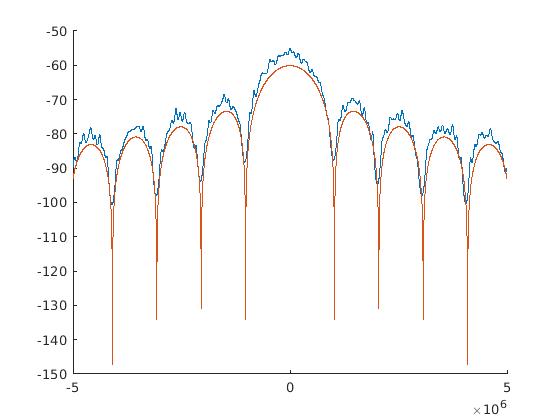
\includegraphics[scale=0.6]{arp100.png}

Error:

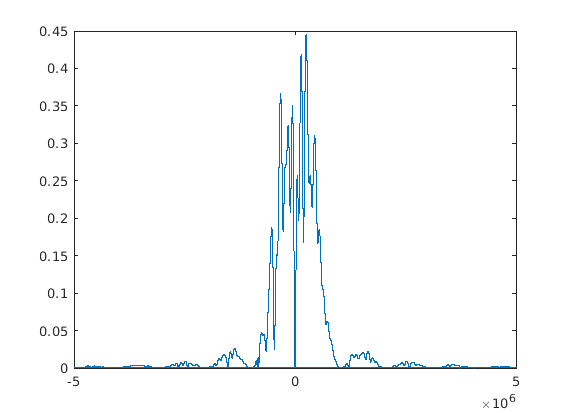
\includegraphics[scale=0.6]{earp100.png}

\subsection{p=1000}
Comparison:

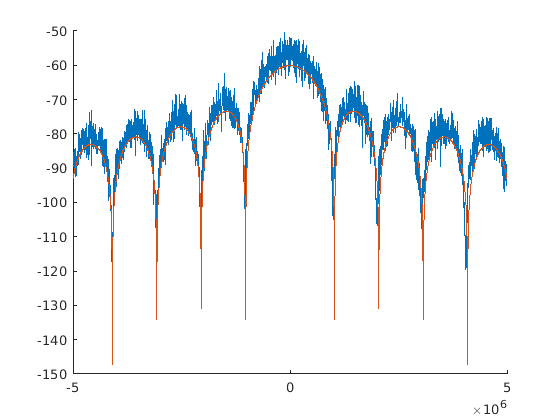
\includegraphics[scale=0.6]{arp1000.png}

Error:

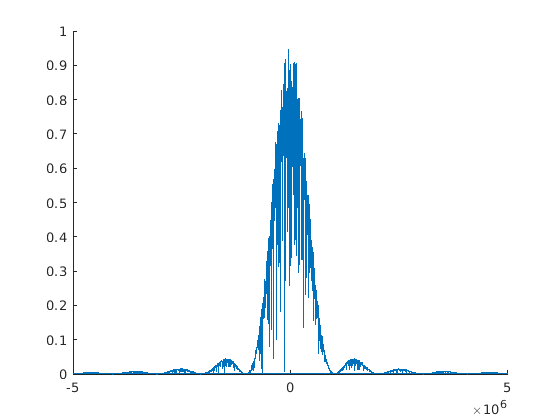
\includegraphics[scale=0.6]{earp1000.png}

As we can appreciate in these graphs, the spectral resolution (and thus the bias) increases with p. This is because when p is low the model that it uses for the signal is simple and it will only be able to fit simple curves, which decreases the frequency resolution (this is also pretty easy to see in the plot of $p=10$, where not many features can be appreciated and only a smooth outline of the result is visible).

In regards to the variance of the errors in the main lobe, we can calculate it using the same code we used previously:

\begin{center}
  \begin{tabular}{ c c }
   p & variance \\
   10 &  0.0051 \\
   100 &  0.0154 \\
   1000 & 0.0805    
  \end{tabular}
\end{center}

It's pretty easy to extrapolate from these results that a higher p results in higher variance. This is because with a higher value of p the model that is being used to simulate the signal gets more complex (since more previous samples are getting used in the estimation of the next one) and therefore the result gets more "wiggly" (if the model is simpler the result is forced to be a simpler function, which makes it smoother and lowers the variance (smoother doesn't directly imply less variance but I'm referring that there's no peaks and sudden changes in the function)).

\section{Appendix}
\subsection{Log plot}
\begin{verbatim}
function log_plot(S, Fs)
    N=length(S);
    x=-Fs/2:Fs/(N-1):Fs/2;
    y=10*log10(fftshift(S));
    plot(x, y)
end
\end{verbatim}

\subsection{Graphs in first section}
\begin{verbatim}
    log_plot(compute_periodogram(RxSignal), Fs)
    genTruePSD(Fs, 1e5, 'GPS', true)
    genTruePSD(Fs, 1e5, 'GPS', true)
    hold on
    log_plot(compute_periodogram(RxSignal), Fs)
    [f, per] = genTruePSD(Fs, 1e5, 'GPS', false);
    log_plot(per, Fs)
\end{verbatim}

\subsection{Graphs in Bias section}
\begin{verbatim}
  plot(fftshift(abs(fft(triang(100)))))
  plot(fftshift(abs(fft(triang(1000)))))
  log_plot(compute_periodogram(RxSignal(1:100)), Fs)
\end{verbatim}

\subsection{Lineal errors}
\begin{verbatim}
function error=compute_error(est, Fs)
  [f, real] = genTruePSD(Fs, 1e5, 'GPS', false);
  real=real./max(real);
  est=est./max(est);
  error=abs(real-est);
end

est=compute_periodogram(RxSignal(1:5000)); % or 5000
plot(f, error);
\end{verbatim}

\subsection{Compute variance}
\begin{verbatim}
  fe=fftshift(error);
  var(fe(4e4:6e4))
\end{verbatim}

\subsection{Barlett's method}
Using a compute\_periodogram function that uses a same-size FFT:
\begin{verbatim}
function S_per = barlett(signal, L)
  agg=[];
  N=length(signal);
  for c=1:N/L:N
    s=signal(c:c+N/L-1);
    per=compute_periodogram(s);
    agg=[agg; per'];
  end
  S_per=mean(agg);
end
\end{verbatim}

\subsection{Barlett graphs}
\begin{verbatim}
 L=2;
 b=barlett(RxSignal, L);
 [f, real] = genTruePSD(Fs, length(b), 'GPS', false);
 hold on
 plot(f, b)
 plot(f, real)
 % Second plot
 error=compute_error(b', Fs)
 plot(f, error)
\end{verbatim}


\subsection{AR graphs}
\begin{verbatim}
   p=1000
   s=compute_AR(RxSignal, p);
   [f, real] = genTruePSD(Fs, length(s), 'GPS', false);
   hold on
   log_plot(s, Fs)
   log_plot(real, Fs)
   % Second plot
   error=compute_error(s, Fs);
   ferror=fftshift(error);
   var(ferror(4e4:6e4))
   plot(f, error)
\end{verbatim}

\end{document}